%!TEX program = xelatex
%!TEX encoding = UTF-8 Unicode
% MpLtX --- a LaTeX Template for Modern Physics Lab
%
%   MpLtX is a template for experiment report of Modern Physics Lab in
% Peking University. 
%
%   Edited by Liang Hao (mail: haoliang@pku.edu.cn), 2016.02.28
%   Change from the template made by Sun Sibai(niasw@pku.edu.cn) 
%   downloaded from http://www.tcep.pku.edu.cn/ 
%   Remove documentclass "revtex4.1", using "article"
%   Change "CJK" to "xeCJK"
%   Test with texlive 2015 in windows 10 and Ubuntu 15.10
%   $xelatex mpltx.tex
%%%%%%%%%%%%%%%%%%%%%%%%%%%%%%%%%%%%%%%%%%%%%%%%%%%%%%%%%%%%%%%
\documentclass[12pt,a4paper]{article}
\usepackage{xeCJK}
\setCJKmainfont[BoldFont={SimHei},ItalicFont={FangSong}]{SimSun}
\setmainfont[ItalicFont={FangSong}]{Times New Roman}
\usepackage{setspace,dcolumn}
\usepackage{subfig}
\usepackage[colorlinks=true]{hyperref}
\usepackage{graphicx,psfrag,epsfig}
\usepackage[font=small,format=plain,labelfont=bf,textfont=it,justification=raggedright,singlelinecheck=false]{caption}
\usepackage{titlesec}
\renewcommand{\thesection}{\Roman{section}}
\renewcommand{\thesubsection}{\Alph{subsection}}
\renewcommand{\thesubsubsection}{\arabic{subsubsection}}
\titleformat*{\section}{\it\large}
\titleformat*{\subsection}{\it\large}
\titleformat*{\subsubsection}{\it\normalsize}
\usepackage{indentfirst}
\setlength{\parindent}{2em}
\usepackage{amsmath,amsfonts,amssymb,amsthm,bm,upgreek}
\usepackage[mathscr]{eucal}
\usepackage{booktabs}
\usepackage{tabularx}
\usepackage[top=2.54cm,bottom=2.54cm,left=3cm,right=3cm]{geometry}

\renewcommand\appendixname{附录}
\renewcommand\abstractname{\vspace{0pt}}%摘要
\renewcommand\tablename{表}
\renewcommand\figurename{图}
\renewcommand\refname{\vspace{0pt}}
\linespread{1.5}
\def\chntoday{\normalsize {\bf 日期: }\the\year~年~\the\month~月~\the\day~日}

\begin{document}

\title{\bf\Large 实验题目}
\author{{\it\large 梁昊\footnote{Email: haoliang@pku.edu.cn; Tel: (86)18811717060}} \\ {\normalsize 北京大学物理学院\quad 学号: 1300011365}}
\date{}%\chntoday}

\maketitle

\abstract
\begin{spacing}{1.5}
此部分为摘要. 200—300字, 说明用什么方法做了什么事, 由此得到什么结果和结论, 有何意义. 摘要中不用缩略词, 不用第一人称.\vspace{20pt}\\
\noindent
{\bf 关键词: } 关键词1, 关键词2, 关键词3, 关键词4 \\ %(2-4个) 
\noindent
{\bf PACS码: }02.10.Yn, 33.15.Vb, 98.52.Cf, 78.47.dc %(选做. 不超过4个,首码须与实验主题一致, PACS(Physics and Astronomy Classification Scheme)代码用于帮助同行检索,可在课程网站下载)
\end{spacing}

\begin{spacing}{2}
\section{要求}
\begin{enumerate}
\item 课程实验报告应假定读者既不是已知全部实验细节的指导教师, 也不是缺少专业知识的公众, 而是同领域的实验研究者, 或审稿人. 不能要求读者要在读过课程讲义后才能读懂课程实验报告.
\item 文本和物理量单位用正体, 物理变量符号用斜体, 矢量矩阵符号用黑斜体.
\item 使用国际标准的缩略词、符号和法定计量单位时应全文一致, 正文中的缩略词在首次出现时写出全称, 后附缩略词, 并用括号括起, 之后直接用缩略词, 不再写全称, 如American Institute of Physics (AIP).
\item 全文标点符号除 “顿号” 外, 其他用英文标点符号.
\item 公式、图和表要分别用阿拉伯数字编列序号. 公式和图表要达到可发表的质量.
\item 凡不是自己独立思考得到的内容都应该引参考文献. 不能大段引用同一参考文献. 对复杂问题, 应该优先考虑引用参考文献得到结果. 对简单一些的问题才鼓励独立思考.
\item 模板中的未尽事项可以参考AIP Style Manual 4th-edition (可从课程网站下载).
\item 较长的推导和说明可以作为附件提交, 不占用报告篇幅.
\item 思考题不是报告的组成部分. 应另起一页附在报告的最后.
\end{enumerate}

\section{引言}
研究论文引言一般包含以下内容: (1)所研究领域背景和现状; (2)有待研究的问题; (3)本研究的目的、主要内容和结果; (6)结果的意义.\par
教学实验肯定不会是原创的. 在写实验报告的引言时, 同学可以假想自己是第一个做类似研究的人.\par
引言一定要切合报告正文, 不能漫无目的地介绍背景. 要快速地将读者引导到报告主题上, 并作较深入的讨论.\par
引言篇幅可以在较大范围内变化, 但最长不应超过报告文字篇幅的1/3.\par
引言撰写可以参考实验讲义, 可以复述, 但不能复制讲义上的任何一句话.\par

\section{实验}
在此部分需要将实验条件交待清楚到别人能重复你的实验结果的程度. 此外,还需表明你已尽了最大努力来提高实验精度和结果的可靠性. 简单的不确定度估计可以在此节给出, 复杂一些的可以放到分析讨论部分.\par
实验条件不仅是指直接影响实验结果的实验参量, 而且还包括影响实验质量和可靠性的因素, 如室温、空气湿度、基真空、原材料纯度等.\par
作为教学实验报告, 此节写详细一点没有坏处.\par
如有必要, 各节下都可以再分节, 如: 
\subsection{实验装置}
\subsubsection{电~源}
\begin{enumerate}
\item {\it 输入变压器} 这是输入变压器. %想用subsubsubsection的自己找解决方案去吧,我懒得写了-lh
\end{enumerate}
...

\section{实验结果及分析讨论}
此部分是实验报告的主体, 应占报告篇幅的一半以上.\par
依自己意愿, 实验结果和对结果的分析讨论既可分为两节也可合在一节.\par
实验结果应尽量以图表的形式给出. 每一个图表都应该是完整的, 即阅读图表时可以不必依赖正文.\par
表是被一系列横线隔开的有序排列的数据, 报告格式要求最上和最下两条横线为双横线. 下页是表格和图片的例子.\par

\begin{table}[htbp]
\caption{这个表格讲述了如何标题, 标题呢, 一般会很长很长很长很长很长很长很长很长的. 这个~}
\label{tab:table1}
\begin{minipage}{\textwidth}
\begin{tabularx}{\textwidth}{ll}
 \hline\hline
  Manucript\footnote{Note a.} & Journals\footnote{Note b.} \\
 \midrule
  {\bf\uppercase\expandafter{\romannumeral 1}.} Principle heading & {\bf\uppercase\expandafter{\romannumeral 1}. principle heading} \\
  A. First subheading & {\bf A. first subheading} \\
  1. Second subheading & {\bf 1. Second subheading} \\
 \hline\hline
\end{tabularx}
\end{minipage}
\end{table}

\begin{figure}[htbp]
\centering
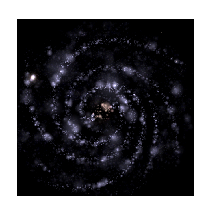
\includegraphics[width=80mm]{Gax}
\caption{噢, 这个是银河吧~图片啊, 标题要自明, 所以也会很长很长很长很长很长很长很长很长的. 这个~}
\label{fig:gax}
\end{figure}
表~\ref{tab:table1} 给出的是 AIP(美国物理联合会)期刊子标题的格式, 我们的对课程报告也作同样的要求.\par
从表~\ref{tab:table1} 可以看出, 对表中各项的注释应作为表的一部分放在表后, 而不是页脚或文尾.\par
每个图一般包含: 图名、轴名、轴、刻度、标尺、数据点、曲线、图例、标注和图注等部分. 应尽量让读者不看正文就能基本理解图的含意.\par
最常用的作图软件是Origin.学习使用基本的数据处理和作图工具软件也是课程的基本内容. 课程鼓励大家使用Python语言编程作图.\par
逐点测量得到的函数关系要同时用表格和图给出. 需要作比较的多条曲线要画在同一图上.\par
为避免读者在图表和正文间反复跳跃阅读, 在正文中也要对图表作必要的说明.\par
公式嘛~TeX专长~
\begin{equation}
N(x_0,y_0,z_0)=\prod_{j\in\{x\}}g(j_0,\sigma^j_0) \label{eq:1}
\end{equation}
对于预料之外的实验结果, 必须首先小心证明其可靠性.读者只有在相信你的实验结果时才愿意花时间看你的分析.\par
必须用文字归纳整理出正式的实验结果或结论.可信的实验结果是课程报告最重要的内容.作为一个实验物理工作者, 分析解释出错并不丢脸, 实验结果不被采信则是致命的.\par
教学实验的结论往往是预先知道的. 所以, 教师更关心的是你的说理过程. 一般说来, 单由课内实验的结果不足以能得到明确的结论. 此时, 你可以引用他人的研究结果来帮助帮助自己的论证, 但必须注明出处. \par
确实不能得到明确结论时, 可以给出几种可能结论并指出可以再做哪些实验来帮助作进一步的判断.\par
总之, 分析讨论部分要做到: 论据要valid, 论证要reasonable, 结论要convincing.\par
\section{结论}
首先要给出实验结果, 然后再给出由实验结果分析得到的结果和结论.此部分给出的内容要比摘要中的全面, 用词要更准确.\par

\section{致谢}
硕、博士论文致谢词产生器 \href{http://acknowledgement.sinaapp.com/}{http://acknowledgement.sinaapp.com/}\\
此部分应感谢指导教师、实验室技术人员、同组人和对实验和报告有帮助的其他人.

\setmainfont{Times New Roman}
\bibliography{bibliography}
%\adcontentsline{toc}{section}{参考文献}
\noindent\rule{.8\textwidth}{1pt}
\begin{thebibliography}{\vspace{0pt}}
\bibitem{Book} 吴思成, 王祖铨~2010 近代物理实验(第三版)(北京: 高等教育出版社)第xxx页.
%
\bibitem{kw1} Chu S, Hollberg L, Bjorkholm J E, Cable A, Ashkin A 1985 {\it Phys. Rev. Lett.} {\bf 55} 8.%%英文期刊
\bibitem{kw2} 耿涛, 闫树斌, 王彦华, 杨海菁, 张天才, 王军民~2005 物理学报~{\bf 54} 5104.%中文期刊
\bibitem{kw3} 王彦华~2007 博士学位论文(太原: 山西大学).%学位论文
\bibitem{kw4} 冯端, 金国钧~2003 凝聚态物理学(上卷)(北京:高等教育出版社) 第341页.%专著
\bibitem{kw5} Tabbal A M, Mérel P, Chaker M 1999 Proceedings of the 14th International Symposium on Plasma Chemistry Prague, Czech Republic, August 2-6, 1999 p1099.%会议文集
\bibitem{kw6} Plank C J U.S. Patent 4 081 490 [1978-02-15].%专利
\bibitem{kw7} 史寒朵~北京大学2012年近代物理实验报告: He-Ne 激光器放电性质研究. %同学实验报告
%
\end{thebibliography}

\clearpage
\appendix
\setmainfont[ItalicFont={FangSong}]{Times New Roman}
\section{思考题}

\end{spacing}
\end{document}
